\documentclass[eng,printmode]{mgr}
%archivemode

\usepackage{polski}
%\usepackage[polish]{babel}
% \usepackage[utf8]{inputenc}
\usepackage[utf8x]{inputenc}
\usepackage[T1]{fontenc}

%pakiety do grafiki
\usepackage{graphicx}
\usepackage{subfigure}
\usepackage{psfrag}
\usepackage{float}
\usepackage{url}
\usepackage{enumitem}
\usepackage{alltt}

% \usepackage{hyperref}
% \hypersetup{colorlinks,urlcolor=blue}

%matematyka
\usepackage{amsmath}
\usepackage{amsfonts}

%tabeli
\usepackage{supertabular}
\usepackage{array}
\usepackage{tabularx}
\usepackage{hhline}
% \usepackage{showlabels}

%kody
\usepackage{listings}
\usepackage{color}
\usepackage{indentfirst}
\usepackage{courier}


\newcommand{\lcolumn}{0.3\textwidth}
\newcommand{\rcolumn}{0.6\textwidth}

\newenvironment{itemize*}%
  {\begin{itemize}%
    \setlength{\itemsep}{0pt}%
    \setlength{\parskip}{0pt}}%
  {\end{itemize}}


\usepackage{array}
\newcolumntype{L}[1]{>{\raggedright\let\newline\\\arraybackslash\hspace{0pt}}m{#1}}
\newcolumntype{C}[1]{>{\centering\let\newline\\\arraybackslash\hspace{0pt}}m{#1}}
\newcolumntype{R}[1]{>{\raggedleft\let\newline\\\arraybackslash\hspace{0pt}}m{#1}}




\definecolor{dkgreen}{rgb}{0,0.6,0}
\definecolor{gray}{rgb}{0.5,0.5,0.5}
\definecolor{mauve}{rgb}{0.58,0,0.82}
\definecolor{mygray}{rgb}{0.5,0.5,0.5}
 
\lstset{ %
  language=c++,                % the language of the code
  basicstyle=\footnotesize\ttfamily, % the size of the fonts that are used for the code
  %numbers=left,                   % where to put the line-numbers
  numberstyle=\tiny\color{gray},  % the style that is used for the line-numbers
  stepnumber=2,                   % the step between two line-numbers. If it's 1, each line 
                                  % will be numbered
  numbersep=5pt,                  % how far the line-numbers are from the code
  backgroundcolor=\color{white},      % choose the background color. You must add \usepackage{color}
  showspaces=false,               % show spaces adding particular underscores
  showstringspaces=false,         % underline spaces within strings
  showtabs=false,                 % show tabs within strings adding particular underscores
  %frame=single,                   % adds a frame around the code
  rulecolor=\color{black},        % if not set, the frame-color may be changed on line-breaks within not-black text (e.g. comments (green here))
  tabsize=2,                      % sets default tabsize to 2 spaces
  captionpos=b,                   % sets the caption-position to bottom
  breaklines=true,                % sets automatic line breaking
  breakatwhitespace=false,        % sets if automatic breaks should only happen at whitespace
  title=\lstname,                   % show the filename of files included with \lstinputlisting;
                                  % also try caption instead of title
  keywordstyle=\color{blue},          % keyword style
  commentstyle=\color{dkgreen},       % comment style
  stringstyle=\color{mauve},         % string literal style
  escapeinside={\%*}{*)},            % if you want to add LaTeX within your code
  morekeywords={*,...},              % if you want to add more keywords to the set
  deletekeywords={...},              % if you want to delete keywords from the given language
  numbers=left,                       % where to put the line-numbers; possible values are (none, left, right)
  numbersep=5pt,                   % how far the line-numbers are from the code
  stepnumber=1,                     %% the step between two line-numbers. If it's 1, each line will be
  numberstyle=\tiny\color{mygray} % the style that is used for the line-numbers
}

\newcommand{\R}{I\!\!R} %symbol liczb rzeczywistych, działa tylko w trybie matematycznym
\newtheorem{theorem}{Twierdzenie}[section] %nowe otoczenie do składania twierdzeń

\title{Obsługa paneli RGB z wykorzystaniem Raspberry~Pi i magistrali SPI lub I²C}
\engtitle{RGB panels control over SPI or I²C interface and Raspberry~Pi}
\author{Mikalai Barysau}
\supervisor{dr inż. Tomasz Surmacz}

\field{Informatyka}
\specialisation{(INS)}

% \DeclareUnicodeCharacter{00A0}{ }

\begin{document}
\bibliographystyle{plabbrv} %tylko gdy używamy BibTeXa, ustawia polski styl bibliografii

\maketitle
%\dedication{6cm}{To jest przykładowa treść opcjonalnej dedykacji, należy ją zmienić lub usunąć w całości polecenie \texttt{$\backslash$dedication}}

\tableofcontents %spis treści

% ************************************************************************************************
%                                           CHAPTER
% ************************************************************************************************
\addcontentsline{toc}{chapter}{\hspace{0.64cm}Wstęp}
\chapter*{Wstęp}

Rosnąca liczba urządzeń elektonicznych w segmencie budżetowym, wzrastające możliwości obliczeniowe komputerów i coraz mniejsze rozmiary processorów, płyt głównych, źródeł zasilania i nośników danych umożliwiają stworzenie produktów, które stosunkowo niedawno wymagały znaczących inwestycji finansowych i zazwyczaj były mało mobilne. 

Obecny świat elektroniczny sprzyja powstaniu licznych ``inteligentnych'' systemów i oddzielnych urządzeń. Niektóre z tych urządzeń już teraz stały się elementami naszego codziennego otoczenia, życia bez których nie możemy sobie wyobrazić. Spad kosztów, wzrost mocy jednostek obliczeniowych i gwałtowne zwiększenie rynku urządzeń elektronicznych powoduje coraz większe zapotrzebowanie społeczności w nowych rozwiązaniach sprzętowych i programowych. 

Warto również zwrócić uwagę na to, że swiąt systemów operacyjnych również bardzo się rozwinął w ciągu ostatnich 20 lat. Jakiś czas temu najbardziej rozpowszechnionym system operacyjnym był system \emph{Microsoft Windows}. Jednak po upływie czasu systemy, oparte na UNIX'ie, takie jak \emph{GNU/Linux} i \emph{OSX}, również zdobyły dużą popularność spośród użytkowników PC, co w tej chwili wymaga od twórców oprogramowania wyboru technologii, które pozwolą na stworzenie narzędzi, które nie będą wymagały od użytkownika zainstalowania dodatkowych biliotek, konifgurowania odpowiedniego środowiska czy jakiejkolwiek ingerecji w process funkcjonowania dostarczonego produktu. Dla użytkownika końcowego najważnieszym jest to, żeby produkt działał w taki sposób, jak od niego się oczekuje. 

Dlatego rola programisty i inżyniera, który jest twórcą tego produktu, polega nie tylko na rozwiązaniu konkretnego problemu technicznego, ale również na przemyśleniu tego, czy dany produkt jest intuicyjny w obsłudze, o ile to jest możliwe, czy on jest sprawny i przetestowany, czy użytkownik końcowy nie będzie w stanie zakłócić działanie programu przez nieodpowiednie korzystanie z dostępnych funkcjonalności.

Stworzenie takiego produktu jest zadaniem nietrywialnym i czasochłonnym. Opracowanie scenariuszy działania tworzonego systemu, przeprowadzenie analizy przypadków użycia, dobór odpowiednich technologii i efektywnych metod obliczeniowych jest niezbędną cześcią procesu tworzenia oprogramowania o wysokiej jakości.

% ************************************************************************************************
%                                           CHAPTER
% ************************************************************************************************
\chapter{Cel pracy}

Celem danej pracy było stworzenie biblioteki do sterowania panelami RGB za pomocą \emph{Raspberry PI} przez interfejs \emph{SPI} oraz aplikacji graficznej, umożliwiającej kalibrowanie kolorów i wykonanie symulacji działania systemu na zwykłym komputerze bez konieczności podłączenia sprzętu. 

Wykorzystany w danej pracy sprzęt wymaga posiadanie pewnej wiedzy technicznej, dotyczącej zasad funkcjonowania pamięci układu \emph{Texas Intruments tlc5947} specyfiki oraz opanowania technik programowania nizkopoziomowego. 

Stworzona bilioteka ma na celu znacznie ułatwić sterowanie podłączonym panelem LED RGB. Uzytkownik biblioteki operuje na obiektach struktury \emph{RGB} i funkcjach, które pozwalają zdefiniować lub pobrać kolor diody o wybranym numerze porządkowym. Dzięki temu nie jest konieczne dokładne zapoznanie się z modelem pamięci sterownika. Dla korzystania z biblioteki potrzebna jest jedynie podstawowa wiedza z programowania w języku \emph{C}. 

Z kolei rozwinięcie biblioteki, lub dostosowanie jej do innego modelu pamięci, będzie wymagało bardziej zaawansowanej wiedzy z dziedziny programowania nizkopoziomowego. Nie powinno to, jednak, być dużym problem, ponieważ jedną z najważniejszych zasad tego projektu było bardzo szczególne dokumentowanie kodu, co pozwala osobie, nie posiadającej niezbędnej wiedzy o układzie \emph{tlc5947}, w stosunkowo krótkim czasie zapoznać się z zasadami operowania na pamięci, definiowania kolorów i wyciągania danych z rejestru presuwnego, wykorzystanego w danym układzie.



% ************************************************************************************************
%                                           CHAPTER
% ************************************************************************************************
\chapter{Opis sprzętu}

\section{Układ \emph{Texas Intruments tlc5947}}
Przy wykonaniu danej pracy został wykorzystany sterownik \emph{Texas Intruments tlc5947} -- 24 kanałowy sterownik diod LED RGB. Każdy z trzech kolorów odpowiada kolorom czerwonomu, zielonemu oraz niebieskiemu.

W środku sterownika znajduje się 36-bajtowy rejestr przesówny. Każdej z ośmiu diod RGB przysługuje 4.5 bajta pamięci, co oznacza że wartość odpowiadająca każdemu kolorowi może mieć wartość w przedziale od \emph{0} do \emph{4095}. 

Specyfika modelu pamięci, zastosowanego w rejestrze przesuwnym układu \emph{Texas Intruments tlc5947}, polega na tym, że dane są uporządkowane w innej kolejności, niż tego może oczekiwać użytkownik. Schemat modelu pamięci jest predstawiony na rysunku \ref{fig:tlc_array}

\begin{figure}[!ht]
    \centering
    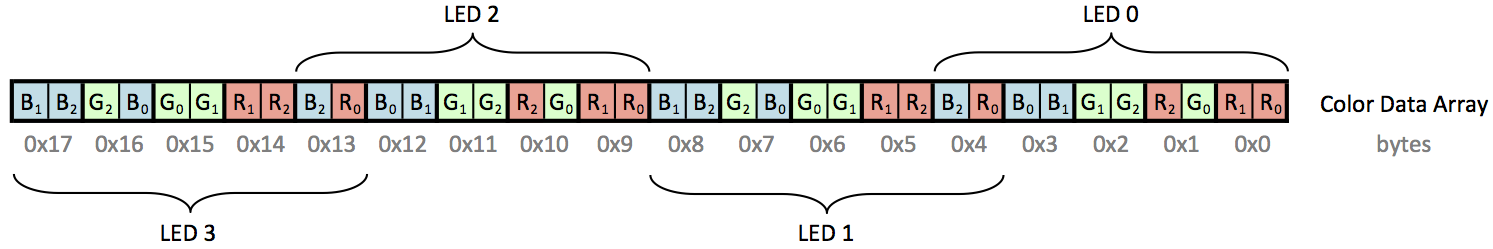
\includegraphics[width=\textwidth]{Figures/tlc_array.png} 
    \caption{Kolejność danych, odpowiadających dwom diodom, w rejestrze przesuwnym sterownika \emph{Texas Intruments tlc5947}}
    \label{fig:tlc_array}
\end{figure}

Litery $R_x G_x B_x$ i kolor komurek odpowiadają kolorom oddzielnej diody. Indeksy~$_x$ oznaczają kolejność liczb szestnastkowych, odpowiadających kodom poszczególnych kolorów. Adresy poszczególnych bajtów wypisane są szarą czcionką. 

Następny przykład (rys. \ref{fig:tlc_2leds}) ilustruje kolejność danych dla 2 diod w dziewięciobajtowym bloku pamięci.

\begin{figure}[!ht]
    \centering
    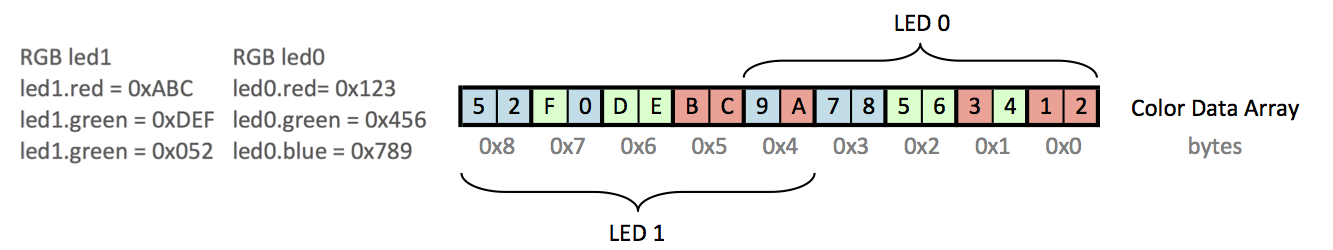
\includegraphics[width=\textwidth]{Figures/tlc_2leds.png} 
    \caption{Kolejność danych, odpowiadających dwom diodom, w rejestrze przesuwnym sterownika \emph{Texas Intruments tlc5947}}
    \label{fig:tlc_2leds}
\end{figure}



\section{Mikrokomputer \emph{Raspberry Pi}}
\emph{Raspberry Pi} -- komputer jednopłytkowy, stworzony przez \emph{Raspberry Pi Foundation}. Mikrokomputer oparty jest na układzie \emph{Broadcom BCM2835 SoC}, który składa się z procesora \emph{ARM1176JZF-S 700 MHz}, \emph{VideoCore IV GPU} i 256 megabajtów (MB) pamięci RAM. Na potrzeby projektu na urządzeniu został zainstalowany system \emph{Raspbian}. 

Konfiguacja programowa mikrokomputera została omówiona w rozdziale \ref{chap:technologies}.

Konfiguracja sprzętowa \emph{Raspberry Pi model B}, który został użyty w danym projekcie, wygląda następująco:


\setlength{\tabcolsep}{10pt} % Default value: 6pt
\renewcommand{\arraystretch}{1.5} % Default value: 1
\vspace{0.5cm}
\begin{tabular}{| m{0.25\textwidth} | m{0.6\textwidth} |}
  \hline             
  \textbf{SoC} & Broadcom BCM2835 (CPU + GPU + DSP + SDRAM) \\ \hline
  \textbf{CPU} & 700 MHz ARM1176JZF-S core (ARM11 family) \\ \hline
  \textbf{GPU} & Broadcom VideoCore IV, OpenGL ES 2.0, 1080p30 h.264/MPEG-4 AVC high-profile decode \\ \hline
  \textbf{Pamięć (SDRAM)} & 256 MB (współdzielona z GPU)  256 MB (współdzielona z GPU) \\ \hline
  \textbf{Porty USB 2.0} & 2 \\ \hline
  \textbf{Nośnik danych} & złącze kart SD / MMC / SDIO MicroSD \\ \hline
  \textbf{Połączenia sieciowe} & 10/100 Ethernet (RJ45) \\ \hline
  \textbf{Pozostałe złącza} & 8 x GPIO, UART, szyna I²C , szyna SPI z dwiema liniami CS, +3,3 V, +5 V, masa \\ \hline
  \textbf{Zasilanie} & 700 mA (3,5 W) \\ \hline
  \textbf{Źródło zasilania} & 5 V przy pomocy złącza MicroUSB, ewentualnie za pomocą złącza GPIO \\ \hline
  \textbf{Wymiary} & 85,60 × 53,98 mm \\ \hline
  \textbf{Waga} & 45 g \\
  \hline  
\end{tabular}




% ************************************************************************************************
%                                           CHAPTER
% ************************************************************************************************

% \addtocounter{chapter}{1}% - ustawi licznik rozdziałów na dwa
\chapter{Opis wybranych technologii}
\label{chap:technologies}

Wybór języka, który będzie głównym narzedziem do realizacji projektu, należy dokonywać biorąc pod uwagę specyfikę projektu, zasoby sprzętowe, przypadki użycia produktu, który powinien powstać, wymagania wydajnościowe oraz funkcjonalne. Niemniej ważny jest czas, którym dysponuje programista. 

Dany projekt jest rozwiązaniem zarówno sprzętowym, jak i programowym. Dlatego wybrane technologie muszą spełniać zestaw określonych wymagań, oraz gwarantować możliwość dalszego utrzymania i rozwoju produktu.

Po przeanalizowaniu najbardziej popularnych obecnie technologii, zostały wybrane języki \emph{C} i \emph{C++} z wykorzystaniem zestawu bibliotek \emph{Qt framework}.

\section{Biblioteka do obsługi układu \emph{Texas Intruments tlc5947}}
Jężyk \emph{C} jest sprawdzonym narzędziem, które pozwala na bardzo szczegółowe manipulacje na pamięci oraz bezpośrednią kontrolę nad złożonością i wydajnością implementowanych funkcji i algorytmów. Język \emph{C++}, z kolei, oprócz wsparcia nizkopoziomowych operacji również pozwala na implementację interfejsów obiektówych i graficznej powłoki do sterowania programem oraz reprezentacji wyników działania i komunikacji z użytkownikiem.


\section{Aplikacja graficzna \emph{LedSimulator} do symulacji działania systemu}
Zaletą języków \emph{C/C++} jest duża wydajność i szybkość wykonywania skompilowanego kodu (pod warunkiem poprawnego posługiwania się możliwościami tych języków, systemu operacyjnego, rejestrami procesora, pamięcią operacyjną i innymi zasobami sprzętowymi). Od momentu stworzenia języków \emph{C} i \emph{C++} została opracowana liczna grupa bibliotek, dających prawie nieograniczone możliwości do tworzenia oprogramowania. Swobodny dostęp do dokumentacji, tutoriali, projektów z otwartym kodem źródłowym i ogromna społeczność programistów \emph{C/C++} jest gwarancją tego, że napotkane problemy techniczne ne zablokują rozwoju produktu i nie pozostawią programistę sam na sam z ich rozwiązaniem.

Jako narzędzie do tworzenia interfejsu graficznego został wybrany \emph{Qt framework}, gdzyż pozwala on w bardzo wygodny sposób tworzyć interfejsy graficzne użytkonika. Oprócz tego \emph{Qt framework} posiada wyjątkowo dobrą dokumentację, która jest wbudowana w IDE \emph{Qt Creator} i również jest dostępna na stronie internetowej projektu \emph{Qt:} 

\begin{alltt}
    \url{http://qt-project.org/doc/}
\end{alltt}

W dokumentacji do framework'u można znaleźć szczegółowe opisy funkcji bibliotecznych i także wiele przykładówych fragmentów kodu, które znacznie ułatwiają rozumienie mechanizmu działania sygnałów i slotów, zasad działanie elementów interfejsu, kontenerów i innych narzędzi bibliotecznych. Kolejną zaletą użycia framework'u \emph{Qt} jest możliwość stworzenia wwieloplatformowej aplikacji graficznej bez konieczności utrzymania kilku wersji kodu dla różnych systemów operacyjnych. 



\section{Programowa konfiguracja \emph{Raspberry Pi}}
Jako środowisko systemowe na \emph{Raspberry Pi} został zainstalowany \emph{Raspbian} -- system operacyjny \emph{GNU/Linux} dla mikrokomputerów \emph{Raspberry Pi}, oparty na dystrybucji \emph{Debian}. Syste, jest dostepny do ściągnięcia z oficjalnej strony projektu \emph{Raspbian}: 

\begin{alltt}
    \url{http://www.raspbian.org/} 
\end{alltt}

lub z oficjalnej strony projektu \emph{Raspberry Pi}:

\begin{alltt}
    \url{http://www.raspberrypi.org/downloads/}
\end{alltt}

Komunikacja z urządzeniami pereferyjnymi przez interfejs \emph{SPI} odbywa się za pomocą sterownika \emph{SPI}, wbudowanego w jądro systemu operacyjnego. Przed rozpoczęciem komunikacji między \emph{Raspberry Pi} i urządzeniem pereferyjnym należy odpowiednio skonfigurować system operacyjny.
Domyślnie sterownik \emph{spi} znajduje się na ``czarnej liście'' modułów jądra systemu i dlatego nie jest ładowany podczas startu systemu.
Aby dodać go do autostartu systemu należy otworzyć plik \emph{/etc/modprobe.d/raspi-blacklist.conf} w edytorze tekstowym i zakomentować linię (umieścić znak `\#' na początku linii), w której znajduje się nazwa sterownika \emph{spi-bcm2708}

\vspace{0.5cm}
\begin{lstlisting}[language=bash,frame=single,caption={Zmodyfikowany plik \emph{/etc/modprobe.d/raspi-blacklist.conf}}]
# blacklist spi and i2c by default (many users don't need them)
# blacklist spi-bcm2708
blacklist i2c-bcm2708
\end{lstlisting}

Również nalezy zmodyfikować plik \emph{/etc/modules}, usuwając znak znać `\#' na początku linii, w której znajduje się nazwa modułu \emph{spi-dev}:
\vspace{0.5cm}

\begin{minipage}{\textwidth}
  \begin{lstlisting}[language=bash,frame=single,caption={Zmodyfikowany plik \emph{/etc/modules}}]
  # /etc/modules: kernel modules to load at boot time.  
  #  
  # This file contains the names of kernel modules that should be loaded  
  # at boot time, one per line. Lines beginning with "#" are ignored.  
  # Parameters can be specified after the module name.  
  #  
  # sound devices  
  snd-bcm2835  
  # SPI devices  
  spi-dev  
  # I2C devices  
  # i2c-dev  
  # 1-Wire devices  
  # w1-gpio  
  # 1-Wire thermometer devices  
  # w1-therm 
  \end{lstlisting} 
\end{minipage}

Po wprowadzeniu zmian należy zrestartować \emph{Raspberry Pi} (np. za pomocą wykonania polecenia \emph{reboot} w linii komend \emph{Raspbian}). 

Po ponownym załadowaniu można sprawdzić, czy moduł \emph{SPI} został załadowany. W tym celu można skorzystać z polecenia \emph{lsmod}.
\vspace{0.5cm}

\begin{minipage}{\textwidth}
  \begin{lstlisting}[language=bash,frame=single,caption={Wynik wykonania polecenia \emph{lsmod}}]
  Module                  Size  Used by
  snd_bcm2835            12808  0
  snd_pcm                74834  1 snd_bcm2835
  snd_seq                52536  0
  snd_timer              19698  2 snd_seq,snd_pcm
  snd_seq_device          6300  1 snd_seq
  snd                    52489  5 snd_seq_device,snd_timer,snd_seq,snd_pcm,snd_bcm2835
  snd_page_alloc          4951  1 snd_pcm
  spidev                  5136  0
  spi_bcm2708             4401  0
  \end{lstlisting} 
\end{minipage}

\section{Interfejs komunikacyjny \emph{SPI}}

Interfejs \emph{SPI} \emph{(Serial Peripheral Interface)} umożliwia komunikację pomiędzy mikrokomputerem i urządzeniem peryferyjnym. Szeregowa transmisja danych odbywa się za pomocą trzech kanałów:

\begin{itemize}
  \item{\emph{\textbf{MOSI} (Master Out / Slave In)} - dane od jednostki nadrzędnej do podporządkowanej}
  \item{\emph{\textbf{MISO} (Master In / Slave Out)} - dane od jednostki podporządkowanej do nadrzędnej}
  \item{\emph{\textbf{SCK} (Serial Clock)} - zegar synchronizujący transmisję}
\end{itemize}

Aktywacją wybranego urządzenia pereferyjnego odbywa się za pomocą dodatkowej linii \emph{\textbf{SS} (Slave Select)}.

Na rysunku \ref{spi} jest umieszczony schemat komunikacji mędzy urządzeniem nadrzędnym i pojedyńczym urządzeniem podporządkowanym.

\begin{figure}[!ht]
    \centering
    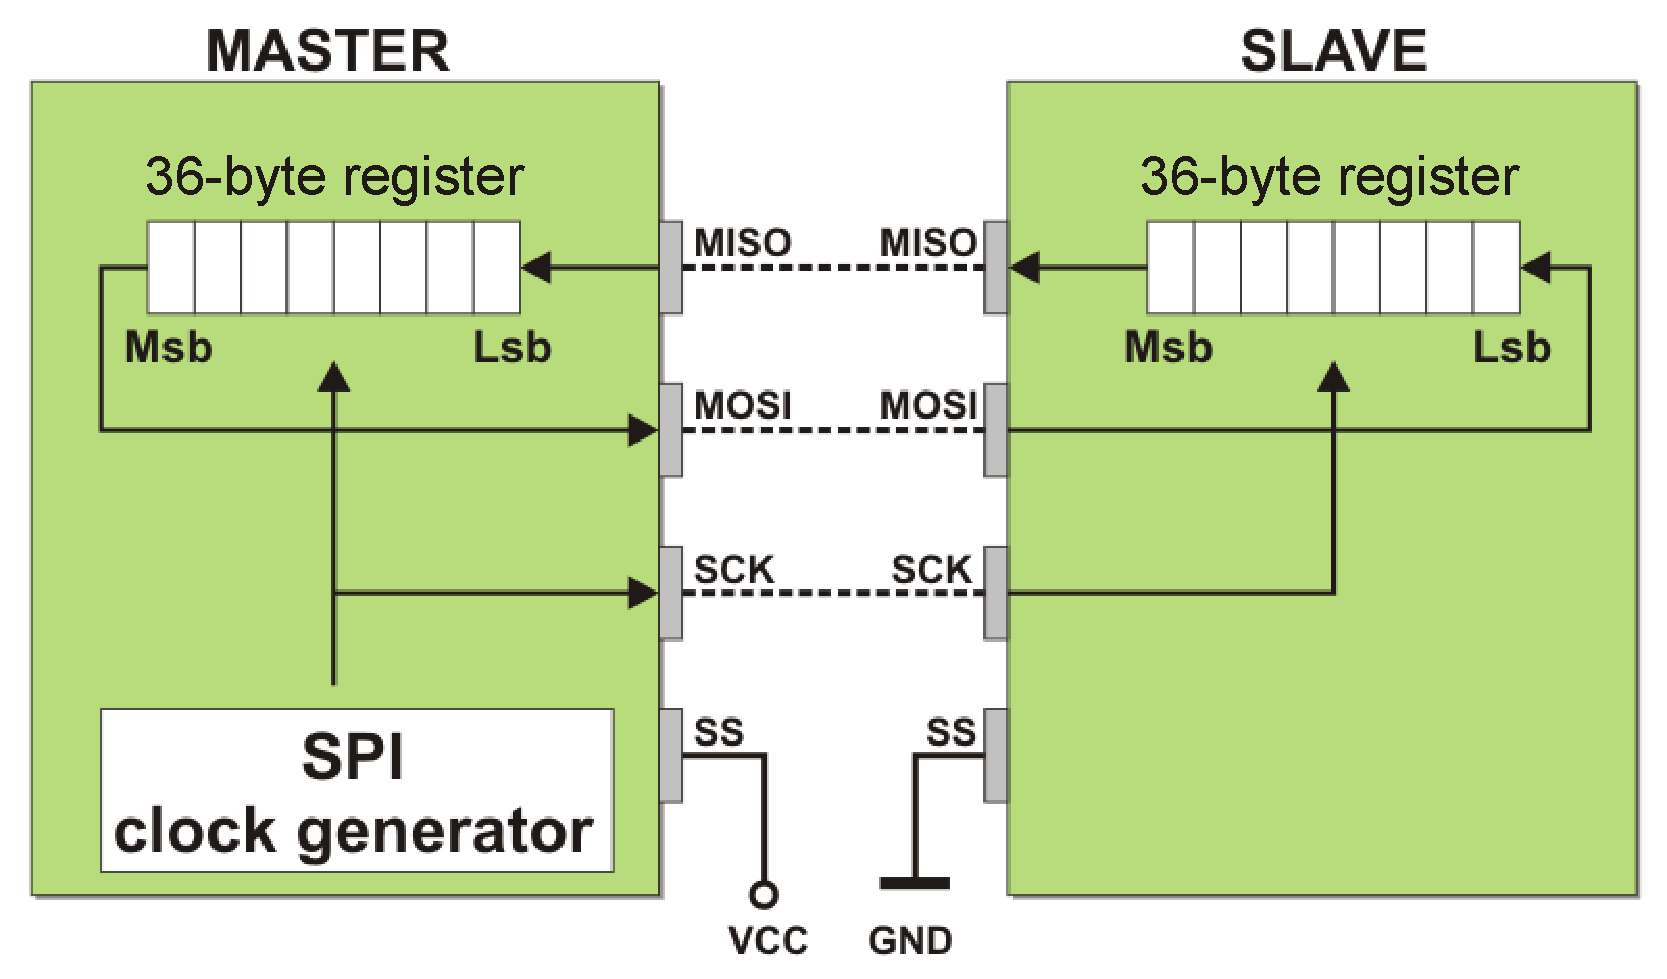
\includegraphics[width=0.7\textwidth]{Figures/spi3.png} 
    \caption{Schemat komunikacji przez interfejs \emph{SPI}}
    \label{spi}
\end{figure}

Po załadowaniu modułów jądra jest możliwa komunikacja z urządzeniem peryferyjnym przez interfejs \emph{SPI}.



% ************************************************************************************************
%                                           CHAPTER
% ************************************************************************************************
\chapter{Implementacja}
\section{Biblioteka do obsługi układu \emph{Texas Intruments tlc5947}}

Biblioteka do sterowania układem składa się z trzech plików:

\begin{itemize}
  \item{\emph{tlc5947\_controller.h}}
  \item{\emph{tlc5947\_controller.c}}
  \item{\emph{RGB.h}}
\end{itemize}

Plik \emph{RGB.h} zawiera structurę \emph{RGB}, która składa się z trzech pól:

\begin{itemize}[before=\ttfamily]
  \item{\textbf{uint64\_t} red}
  \item{\textbf{uint64\_t} green}
  \item{\textbf{uint64\_t} blue}
\end{itemize}

Każde pole służy do przechowywania wartości odpowiedniego koloru. Struktura została przeniesiona do oddzielnego pliku w cela dalszej możliwości korzystania z nej bez konieczności dołączania całej biblioteki.

\vspace{0.3cm}

Plik nagłówkowy \emph{tlc5947\_controller.h} zawiera makro definicje i nagłówki trzech funkcji, które stanowią interfejs zewnętrzny (API) biblioteki:

\begin{itemize}[before=\ttfamily]
  \item{\textbf{int} setLedRGB(\textbf{uint32\_t} ledNumber, \textbf{RGB} rgbSet, \textbf{uint8\_t*} tab)}
  \item{\textbf{RGB} getLedRGB(\textbf{uint8\_t} ledNumber, \textbf{uint8\_t*} tab)}
  \item{\textbf{void} printLedDataArray(\textbf{uint8\_t*} tab)}
\end{itemize}

Również pllik \emph{tlc5947\_controller.h} zawiera krótki komentarz, który wyjaśnia zasadę indeksowania diod w rejestrze przesuwnym układu \emph{Texas Instruments tlc5947}. 

\vspace{0.3cm}

%\begin{minipage}{\textwidth}
Plik \emph{tlc5947\_controller.c} oprócz implementacji interfejsu zawiera również implementacje funkcji statycznych, które nie są widoczne dla użytkownika biblioteki, natomiast są wykorzystywane w mechanizmach adresacji i komunikacji z układem \emph{tlc5947}. Lista zaimplementowanych funkcji wygląda nastepująco:


  \begin{itemize}[before=\ttfamily]
    \item{\textbf{static void} cleanRGB(\textbf{RGB*} rgb)}
    \item{\textbf{static uint64\_t} getLedIndex(\textbf{uint8\_t} ledNumber)} 
    \item{\textbf{static uint64\_t} compileEvenLedPattern(\textbf{RGB} rgbSet)} 
    \item{\textbf{static uint64\_t} compileOddLedPattern(\textbf{RGB} rgbSet)} 
    \item{\textbf{static int} insertLedRgb(\textbf{uint32\_t} ledNumber, \textbf{uint64\_t} RGBpattern, \textbf{uint8\_t*} tab)} 
    \item{\textbf{RGB} getLedRGB(\textbf{uint8\_t} ledNumber, \textbf{uint8\_t*} tab)} 
    \item{\textbf{int} setLedRGB(\textbf{uint32\_t} ledNumber, \textbf{RGB} rgbSet, \textbf{uint8\_t*} tab)} 
    \item{\textbf{void} printLedDataArray(\textbf{uint8\_t*} tab)} 
  \end{itemize}
%\end{minipage}

\vspace{0.7cm}

W dalszej części tego rozdziału przedstawiony jest szczegółowy opis funkcji z przykładami kodu.
% \clearpage

%---------------function
\subsection{cleanRGB} 
%\begin{minipage}{\textwidth}

%description
Funkcja służy do czyszczenia obiektu struktury \emph{RGB}.
%description

\begin{center}
  \begin{tabular}{|L{\lcolumn}|L{\rcolumn}|}
    \hline
    
    \textbf{Nazwa funkcji}  & \textit{
        cleanRGB
        } \\ \hline
        
    \textbf{Funkcja statyczna} & 
        tak
        \\ \hline
        
    \textbf{Parametry wejściowe}  & 
        \emph{\textbf{RGB*} rgb} -- wskaźnik na obiekt struktury \emph{RGB}
        \\ \hline
        
    \textbf{Parametry wyjściowe} &
        --
        \\ \hline
        
  \end{tabular}
\end{center}
%\end{minipage}
\vspace{0.5cm}
%---------------function


%---------------function
\subsection{getLedIndex} 
%\begin{minipage}{\textwidth}

%description
Funkcja służy do obliczania indeksu bloku pamięci diody w rejestrze przesuwnym. W związku z tym. Dzięki tej funkcji użytkownik biblioteki nie musi uwzględniać modelu pamięci rejestru przesuwnego układu \emph{tlc5947}, korzystając z niego tak samo, jak ze zwykłej tablicy bajtowej. 
%description

\begin{center}
  \begin{tabular}{|L{\lcolumn}|L{\rcolumn}|}
    \hline
    
    \textbf{Nazwa funkcji}  & \textit{
        getLedIndex
        } \\ \hline
        
    \textbf{Funkcja statyczna} & 
        tak
        \\ \hline
        
    \textbf{Parametry wejściowe}  & 
        \emph{\textbf{uint8\_t} ledNumber} -- numer diody
        \\ \hline
        
    \textbf{Parametry wyjściowe} &
        \emph{\textbf{uint64\_t} ledAddress} -- indeks początku bloku pamięci diody w rejestrze przesuwnym
        \\ \hline
        
  \end{tabular}
\end{center}
%\end{minipage}
\vspace{0.5cm}
%---------------function


%---------------function
\subsection{compileOddLedPattern} 
%\begin{minipage}{\textwidth}

%description
Funkcja służy do kompilacji fragmentu pamięci dla diody o numerze nieparzystym, który będzie zawierał uporządkowane w odpowiedniej kolejności wartości dla kolorów czerwonego, zielonego i niebieskiego.
Przykład działania funkcji:
W przypadku, gdy Parametr wejsciowy \emph{\textbf{RGB} rgbSet} ma nastepujace wartosci:

\begin{itemize}
  \item{rgbSet.red   = 0x123}
  \item{rgbSet.green = 0x456}
  \item{rgbSet.blue  = 0x789}
\end{itemize}
             
Funkcja zwróci wartość 64-bitową, która stanowi następujący fragment pamięci:

\vspace{0.3cm}
\hspace{0.3cm} \textbf{[00 00 00 89 67 45 23 01]}
\vspace{0.3cm}

Otrzymany w wyniku fragmnet jest później wkładany do tablicy \emph{txdata}, która jest przesyłana do rejestru przesuwnego. Z tego powodu, że otzymany fragment pamięci jest wkładany do tablicy \emph{txdata} za pomocą operacji logicznej \emph{OR}, wartości dla odpowiednich kolorów znajdują się na właściwych pozycjach, reszta fragmentu pamięci jest wypełniona zerami, żeby nie zmodyfikować wartości kolorów dla innych diod, które znajdują się w tablicy.

Operację na pamięci w większości wykonywane są za pomoća operatorów logicznych \emph{AND}, \emph{OR} oraz przesunięć bitowych. W kodzie biblioteki znajduje się szczegółowy opis zmian, które odbywają się w pamięci.

\vspace{0.3cm}
\begin{lstlisting}[language=c,frame=single,caption={Fragment kodu, w którym przedstawiony jest komentarz ilustrujący efekt wykonywania operacji na pamięci}]
  //compiling green color     
  hex = 0;                    //     hex = [00 00 00 00 00 00 00 00]
  hex = green & hex1Mask;     //     hex = [00 00 00 00 00 00 04 00]
  hex = hex << 3 * POSITION;  //     hex = [00 00 00 00 00 40 00 00]
  pattern = pattern | hex;    // pattern = [00 00 00 00 00 40 23 01]

\end{lstlisting}

%description


\begin{center}
  \begin{tabular}{|L{\lcolumn}|L{\rcolumn}|}
    \hline
    
    \textbf{Nazwa funkcji}  & \textit{
        compileEvenLedPattern
        } \\ \hline
        
    \textbf{Funkcja statyczna} & 
        tak
        \\ \hline
        
    \textbf{Parametry wejściowe}  & 
        \emph{\textbf{RGB} rgbSet} -- obiek struktury \emph{RGB}, który zawiera wartości dla odpowiednich kolorów
        \\ \hline
        
    \textbf{Parametry wyjściowe} &
        \emph{\textbf{uint64\_t} pattern} -- spreparowany fragment pamięci, który następnie zostanie włożony do rejestru presuwnego
        \\ \hline
        
  \end{tabular}
\end{center}
%\end{minipage}
\vspace{0.5cm}
%---------------function



%---------------function
\subsection{compileEvenLedPattern} 
%\begin{minipage}{\textwidth}

%description
Funkcja służy do kompilacji fragmentu pamięci dla diody o numerze parzystym, który będzie zawierał uporządkowane w odpowiedniej kolejności wartości dla kolorów czerwonego, zielonego i niebieskiego.
Przykład działania funkcji:
W przypadku, gdy Parametr wejsciowy \emph{\textbf{RGB} rgbSet} ma nastepujace wartosci:

\begin{itemize}
  \item{rgbSet.red   = 0x123}
  \item{rgbSet.green = 0x456}
  \item{rgbSet.blue  = 0x789}
\end{itemize}
             
Funkcja zwróci wartość 64-bitową, która stanowi następujący fragment pamięci:

\vspace{0.3cm}
\hspace{0.3cm} \textbf{[00 00 00 90 78 56 34 21]}
\vspace{0.3cm}

Otrzymany w wyniku fragmnet jest później wkładany do tablicy \emph{txdata}, która jest przesyłana do rejestru przesuwnego. Z tego powodu, że otzymany fragment pamięci jest wkładany do tablicy \emph{txdata} za pomocą operacji logicznej \emph{OR}, wartości dla odpowiednich kolorów znajdują się na właściwych pozycjach, reszta fragmentu pamięci jest wypełniona zerami, żeby nie zmodyfikować wartości kolorów dla innych diod, które znajdują się w tablicy.

Operację na pamięci w większości wykonywane są za pomoća operatorów logicznych \emph{AND}, \emph{OR} oraz przesunięć bitowych. W kodzie biblioteki znajduje się szczegółowy opis zmian, które odbywają się w pamięci.

\vspace{0.3cm}
\begin{lstlisting}[language=c,frame=single,caption={Fragment kodu, w którym przedstawiony jest komentarz ilustrujący efekt wykonywania operacji na pamięci}]
  //compiling blue color    
  hex = 0;                    //     hex = [00 00 00 00 00 00 00 00]
  hex = blue & hex1Mask;      //     hex = [00 00 00 00 00 00 07 00]
  hex = hex << 5 * POSITION;  //     hex = [00 00 00 00 70 00 00 00]
  pattern = pattern | hex;    // pattern = [00 00 00 00 70 56 34 12]

\end{lstlisting}

%description


\begin{center}
  \begin{tabular}{|L{\lcolumn}|L{\rcolumn}|}
    \hline
    
    \textbf{Nazwa funkcji}  & \textit{
        compileEvenLedPattern
        } \\ \hline
        
    \textbf{Funkcja statyczna} & 
        tak
        \\ \hline
        
    \textbf{Parametry wejściowe}  & 
        \emph{\textbf{RGB} rgbSet} -- obiek struktury \emph{RGB}, który zawiera wartości dla odpowiednich kolorów
        \\ \hline
        
    \textbf{Parametry wyjściowe} &
        \emph{\textbf{uint64\_t} pattern} -- spreparowany fragment pamięci, który następnie zostanie włożony do rejestru presuwnego
        \\ \hline
        
  \end{tabular}
\end{center}
%\end{minipage}
\vspace{0.5cm}
%---------------function



%---------------function
\subsection{insertLedRgb} 
%\begin{minipage}{\textwidth}

%description
Funkcja służy do obliczania indeksu bloku pamięci diody w rejestrze przesuwnym. W związku z tym. Dzięki tej funkcji użytkownik biblioteki nie musi uwzględniać modelu pamięci rejestru przesuwnego układu \emph{tlc5947}, korzystając z niego tak samo, jak ze zwykłej tablicy bajtowej. 
%description

\begin{center}
  \begin{tabular}{|L{\lcolumn}|L{\rcolumn}|}
    \hline
    
    \textbf{Nazwa funkcji}  & \textit{
        insertLedRgb
        } \\ \hline
        
    \textbf{Funkcja statyczna} & 
        tak
        \\ \hline
        
    \textbf{Parametry wejściowe}  & 
        \begin{itemize}
        \item{\emph{\textbf{uint32\_t} ledNumber} -- number diody, której dotyczy działanie} 
        \item{\emph{\textbf{uint64\_t} RGBpattern} -- spreparowany 64-bitowy fragment pamięci, zawierający odpowiednie wartości kolorów} 
        \item{\emph{\textbf{uint8\_t*} tab} -- wskaźnik na tablicę \emph{txdata}, która zostanie później przesłana do rejestru przesuwnego} 
        \end{itemize}
        \\ \hline
        
    \textbf{Parametry wyjściowe} &
        \emph{\textbf{int}} -- wartość \emph{0} mówi o skutecznym wykonaniu operacji; w przypadku błędu zwracana jest wartość \emph{-1}
        \\ \hline
        
  \end{tabular}
\end{center}
%\end{minipage}
\vspace{0.5cm}
%---------------function



%---------------function
\subsection{getLedRGB} 
%\begin{minipage}{\textwidth}

%description
Funkcja zwraca obiekt struktury \emph{\textbf{RGB}}, który zawiera wartości kolorów wybranej diody. Wartości są pobierane z tablicy \emph{txdata}, i wyciągane za pomocą operatorów logicznych \emph{AND}, \emph{OR} oraz przesunięć bitowych. W kodzie biblioteki znajduje się szczegółowy opis zmian, które odbywają się w pamięci.

\vspace{0.3cm}
\begin{lstlisting}[language=c,frame=single,caption={Fragment kodu, w którym przedstawiony jest komentarz ilustrujący efekt wykonywania operacji na pamięci}]
  //getting red color
  hex = pattern & (0x0F);        //        hex = [00 00 00 00 00 00 00 01]
  hex = hex << 2 * POSITION;     //        hex = [00 00 00 00 00 00 01 00]
  ledRGB.red = ledRGB.red | hex; // ledRgb.red = [00 00 00 00 00 00 01 00]
  hex = 0;                       //        hex = [00 00 00 00 00 00 00 00]

\end{lstlisting}
%description

\begin{center}
  \begin{tabular}{|L{\lcolumn}|L{\rcolumn}|}
    \hline
    
    \textbf{Nazwa funkcji}  & \textit{
        getLedRGB
        } \\ \hline
        
    \textbf{Funkcja statyczna} & 
        nie
        \\ \hline
        
    \textbf{Parametry wejściowe}  & 
        \begin{itemize}
        \item{\emph{\textbf{uint32\_t} ledNumber} -- number diody, której dotyczy działanie} 
        \item{\emph{\textbf{uint64\_t} RGBpattern} -- spreparowany 64-bitowy fragment pamięci, zawierający odpowiednie wartości kolorów} 
        \item{\emph{\textbf{uint8\_t*} tab} -- wskaźnik na tablicę \emph{txdata}, która zostanie później przesłana do rejestru przesuwnego} 
        \end{itemize}
        \\ \hline
        
    \textbf{Parametry wyjściowe} &
        \emph{\textbf{RGB} ledRGB} -- obiekt struktury \emph{\textbf{RGB}}, który zawiera odpowiednie wartości kolorów czerwonego, zielonego i niebieskiego wybranej diody
        \\ \hline
        
  \end{tabular}
\end{center}
%\end{minipage}
\vspace{0.5cm}
%---------------function



%---------------function
\subsection{setLedRGB} 
%\begin{minipage}{\textwidth}

%description
Funkcja służy do ustawiana koloru wybranej diody. Funkcja korzysta z funkcji statycznych biblioteki: \emph{compileEvenLedPattern}, \emph{compileOddLedPattern}, \emph{insertLedRgb}
%description

\begin{center}
  \begin{tabular}{|L{\lcolumn}|L{\rcolumn}|}
    \hline
    
    \textbf{Nazwa funkcji}  & \textit{
        setLedRGB
        } \\ \hline
        
    \textbf{Funkcja statyczna} & 
        nie
        \\ \hline
        
    \textbf{Parametry wejściowe}  & 
        \begin{itemize}
        \item{\emph{\textbf{uint32\_t} ledNumber} -- number diody, której dotyczy działanie} 
        \item{\emph{\textbf{RGB} rgbSet} -- obiekt struktury \emph{\textbf{RGB}}, który zawiera odpowiednie wartości kolorów czerwonego, zielonego i niebieskiego} 
        \item{\emph{\textbf{uint8\_t*} tab} -- wskaźnik na tablicę \emph{txdata}, która zostanie później przesłana do rejestru przesuwnego} 
        \end{itemize}
        \\ \hline
        
    \textbf{Parametry wyjściowe} &
        \emph{\textbf{int} result} -- wartość \emph{0} mówi o skutecznym wykonaniu operacji; w przypadku błędu zwracana jest wartość \emph{-1}
        \\ \hline
        
  \end{tabular}
\end{center}
%\end{minipage}
\vspace{0.5cm}
%---------------function



%---------------function
\subsection{setLedRGB} 
%\begin{minipage}{\textwidth}

%description
Funkcja służy do wyświetlania zawartości tablicy \emph{txdata} na standardowym wyjściu.
%description

\begin{center}
  \begin{tabular}{|L{\lcolumn}|L{\rcolumn}|}
    \hline
    
    \textbf{Nazwa funkcji}  & \textit{
        printLedDataArray
        } \\ \hline
        
    \textbf{Funkcja statyczna} & 
        nie
        \\ \hline
        
    \textbf{Parametry wejściowe}  & 
        \emph{\textbf{uint8\_t*} tab} -- wskaźnik na tablicę \emph{txdata}, która zawiera wartości kolorów wszystkich diod
        \\ \hline
        
    \textbf{Parametry wyjściowe} &
        --
        \\ \hline
        
  \end{tabular}
\end{center}
%\end{minipage}
\vspace{0.5cm}
%---------------function


% ************************************************************************************************
%                                           Section
% ************************************************************************************************
\section{Aplikacja graficzna \emph{LedSimulator}}




\begin{figure}[!ht]
    \centering
    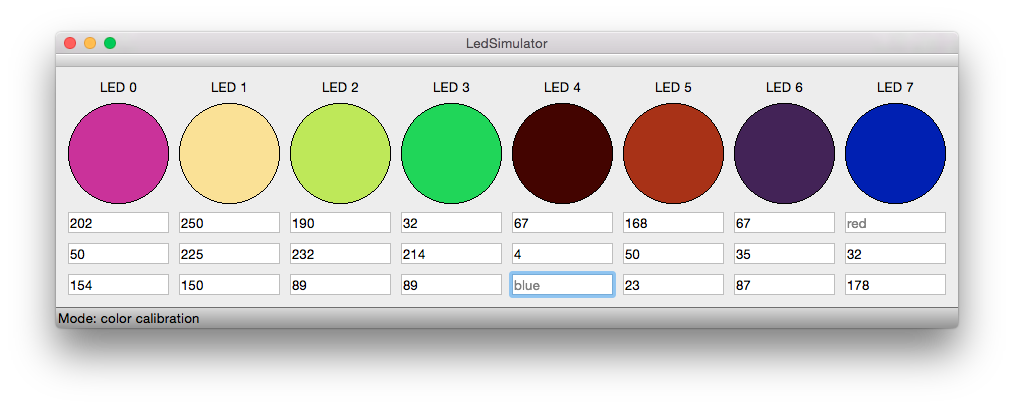
\includegraphics[width=\textwidth]{Figures/ledSimulator.png} 
    \caption{Aplikacja graficzna \emph{LedSimulator}: przykładowe kolory}
    \label{fig:ledSimulator}
\end{figure}


Na podanym zrzucie ekranu (rys. \ref{fig:ledSimulator}) jest przedstawione okno główne alikacji graficznej \emph{LedSimulator}. Aplikacja znajduje się w trybie \emph{Color calibration}. Pokazany jest układ zawierający 8 diod RGB. Diody są ponumerowane od \emph{0}. Każdej diodzie przysługują 3 pola tekstowe:

\begin{itemize}
  \item{\emph{red}}
  \item{\emph{green}}
  \item{\emph{blue}}
\end{itemize}

W każde pole użytkownik może wprowadzić wartość od \emph{0} do \emph{255}. Wprowadzane wartości są sprawdzane za pomocą wyrażeń regularnych, dzięki czemu nie jest możliwe wprowadzenie innych znaków, niż cyfry, oraz liczb, większych niż 255.

Kolory diod są odświeżane w momencie zmiany wartości w odpowiednim polu. Domyślną wartością, przechowywaną w każdym polu, jest \emph{0}, co oznacza brak koloru (rys. \ref{fig:ledSimulator2}).

\begin{figure}[!ht]
    \centering
    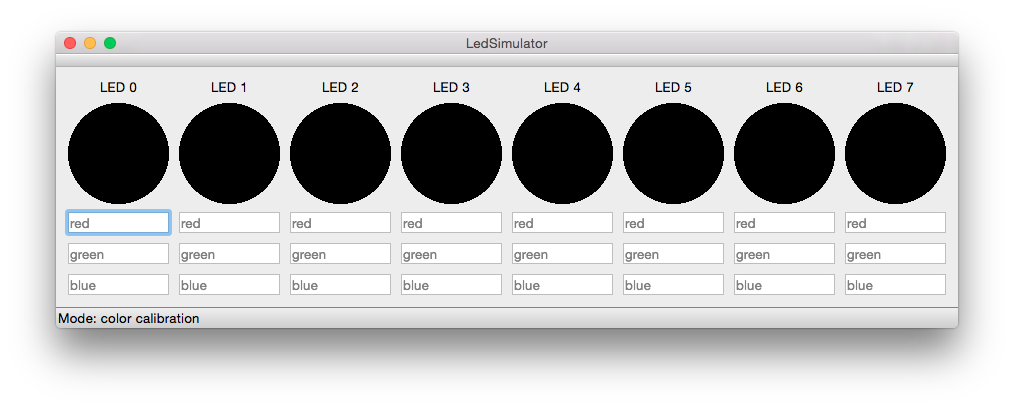
\includegraphics[width=\textwidth]{Figures/ledSimulator2.png} 
    \caption{Aplikacja graficzna \emph{LedSimulator}: domyślny stan diod}
    \label{fig:ledSimulator2}
\end{figure}


Aplikacja może pracować w dwóch trybach (rys. \ref{fig:modes}):

\begin{itemize}
  \item{\emph{Color calibration}}
  \item{\emph{TLC5947 simulation}}
\end{itemize}

Tryb \emph{Color calibration} został opisany wyżej.

Tryb \emph{TLC5947 simulation} służy do testowania działania biblioteki w przypadku braku dostępu do układu \emph{Texas Instruments TLC5947}. Przy wyborze tego trybu uruchomiony zostanie scenariusz, umieszczony w funckcji \emph{runLedScenario}. 

\begin{figure}[!ht]
    \centering
    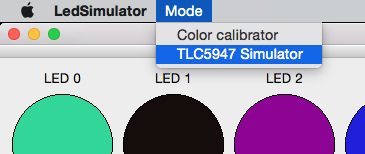
\includegraphics[width=0.5\textwidth]{Figures/modes.png} 
    \caption{Wybór trybu działania aplikacji \emph{LedSimulator}}
    \label{fig:modes}
\end{figure}


%opcjonalnie możliwe tu pojawienie spis rysunków i tabel
\addcontentsline{toc}{chapter}{\hspace{0.64cm}\listfigurename}
\listoffigures
% \listoftables

\newpage
\renewcommand{\thechapter}{}
\renewcommand{\chaptername}{}
\chapter{Literatura}
\begin{enumerate}
%\item Strona internetowa \hyperref{http://journals.bg.agh.edu.pl/AUTOMATYKA/\2006-03/Auto_531-542.pdf}

\item {A. Janiak, \emph{Wybrane problemy i algorytmy szeregowania  zadań i rozdziału zasobów}, Warszawa: Akademicka Oficyna Wydawnicza PLJ 1999}

\item {Strona internetowa: \url{http://en.wikipedia.org/wiki/Job-shop_scheduling}, 08.10.2014}

\item {M. Sobolewski, \url{http://www.ioz.pwr.wroc.pl/pracownicy/kuchta/Marek%20Sobolewski_FlowShop.pdf}, 08.10.2014}

\item {C. Smutnicki, \emph{Algorytmy szeregowania zadań}, \url{http://www.kierunkizamawiane.pwr.wroc.pl/materialy/smut.pdf}, 08.10.2014}

\item {Lekcja \emph{The Knapsack Problem}, \url{http://www.es.ele.tue.nl/education/5MC10/Solutions/knapsack.pdf}, 08.10.2014}

\item {Strona internetowa: \url{http://en.wikipedia.org/wiki/Knapsack_problem}, 08.10.2014}

\item {D. Pisinger, \emph{Algorithms For Knapsack Problems}, \url{http://www.diku.dk/~pisinger/95-1.pdf}, 08.10.2014}

\item {Strona internetowa: \url{http://en.wikipedia.org/wiki/Travelling_salesman_problem}, 08.10.2014}

\item {Shen Lin, \emph{Computer Solutions of the Traveling Salesman Problem}, \url{http://alcatel-lucent.com/bstj/vol44-1965/articles/bstj44-10-2245.pdf}, 08.10.2014}

\item {John D. C. Little, Katta G. Murty, Dura W. Sweeney, Caroline Karel, \emph{An algorithm for the traveling salesman problem}, \url{http://dspace.mit.edu/bitstream/handle/1721.1/46828/algorithmfortrav00litt.pdf}, 08.10.2014}

\item {Strona internetowa: \url{http://www.princeton.edu/~achaney/tmve/wiki100k/docs/Travelling_salesman_problem.html}, 08.10.2014}

\item {Strona internetowa: \url{http://qt-project.org/doc/}, 08.10.2014}

\end{enumerate}
\end{document}

\end{document}